\documentclass[a4paper,12pt, twoside]{article}
\usepackage[a4paper, left=2.5cm, right=2.5cm, top=2.5cm, bottom=2.5cm, bindingoffset=0.5cm]{geometry}
\usepackage[utf8x]{inputenc}
\usepackage{polski}
\usepackage[polish]{babel}
\usepackage{graphicx}
\usepackage{indentfirst}
\usepackage{float}
\usepackage{caption}
\usepackage{adjustbox}
\usepackage{array}
\usepackage{makecell}
\usepackage{amsmath}
\usepackage{enumitem}
\usepackage{afterpage}
\usepackage{subfig}
\usepackage{hyperref}
\usepackage{url}
\usepackage{listings}
\usepackage{xcolor}

%New colors defined below
\definecolor{codegreen}{rgb}{0,0.6,0}
\definecolor{codegray}{rgb}{0.5,0.5,0.5}
\definecolor{codepurple}{rgb}{0.58,0,0.82}
\definecolor{backcolour}{rgb}{0.95,0.95,0.92}

%Code listing style named "mystyle"
\lstdefinestyle{mystyle}{
  backgroundcolor=\color{backcolour},   commentstyle=\color{codegreen},
  keywordstyle=\color{magenta},
  numberstyle=\tiny\color{codegray},
  stringstyle=\color{codepurple},
  basicstyle=\ttfamily\footnotesize,
  breakatwhitespace=false,         
  breaklines=true,                 
  captionpos=b,                    
  keepspaces=true,                 
  numbers=left,                    
  numbersep=5pt,                  
  showspaces=false,                
  showstringspaces=false,
  showtabs=false,                  
  tabsize=2
}

\lstset{style=mystyle}


\renewcommand\thesection{\arabic{section}.}
\renewcommand\thesubsection{\arabic{section}.\arabic{subsection}.}
\renewcommand\thesubsubsection{\arabic{section}.\arabic{subsection}.\arabic{subsubsection}.}
\renewcommand{\lstlistingname}{Algorytm}% Listing -> Algorithm
\frenchspacing
\setlength{\parindent}{.5cm}
\makeatletter
\setlength{\@fptop}{0pt}
\makeatother
\linespread{1.5}
\begin{document}
	\newpage
	\thispagestyle{empty}
	\begin{center}
		
		\begin{figure}
			\centering
			
\includegraphics[width=7cm]{images/polsl_logo.jpg}
			\vspace{.5cm}
		\end{figure}
		
		{\fontsize{17}{17}\selectfont
			\textsc{Politechnika Śląska \\[.3cm]
				Wydział Automatyki, Elektroniki i Informatyki  \\[.3cm]
				Kierunek Automatyka i Robotyka  \\[1.5cm]}
			\textbf{Projekt inżynierski \\[0.7cm]}}
		
		\Large
		{Elektroniczna plakietka konfigurowana z urządzenia mobilnego \\[3.5cm]}
		\Large{\begin{flushleft}
				Autor: Jakub Legutko\\
				Kierujący pracą: dr inż. Grzegorz Dziwoki\\[0.3cm]
		\end{flushleft}}
		
		\normalsize
		\vfill Gliwice, styczeń 2020
	\end{center}
	\newpage
	\newpage
	\thispagestyle{empty}
	\tableofcontents
	\newpage
	%\leavevmode\thispagestyle{empty}\newpage
	\newpage
	\clearpage
	\setcounter{page}{1}
	
	\section{Wstęp}
	
	\subsection{Wprowadzenie}
	Zmiany klimatyczne są coraz bardziej widoczne na świecie. Wycinka drzew jest jednym z głównych powodów wzrostu emisji gazów cieplarnianych\cite{clima_causes}, ograniczenie jej wpłynie pozytywnie na poziom ${CO_{2}}$ w atmosferze, co przełoży się na polepszenie klimatu. 
	
	Druk wizytówek oraz identyfikatorów pochłania znaczące ilości papieru, oraz tuszu w skali globalnej ze względu na ich jednorazowe wykorzystanie w większości przypadków. Z tego powodu ważne jest znalezienie alternatywnej metody. Gdyby zamiast papieru wykorzystać urządzenie, z którego można korzystać wielokrotnie poprzez zmianę wyświetlanych danych, zmniejszylibyśmy zapotrzebowanie na papier, zmniejszając jednocześnie emisję dwutlenku węgla. Oprócz papieru potrzebnego do wytworzenia plakietek nie będziemy również marnować toneru, którego produkcja pochłania około 3.2 kilograma gazów cieplarnianych\cite{cartidge_production} na kartridż zawierający 200 gramów toneru. Kolejną rzeczą jest recykling, któremu trzeba poddać niepotrzebne już identyfikatory oraz zużyte do produkcji ich kartridże.
	
	Idealnym rozwiązaniem takiego problemu wydaje się papier elektroniczny (ang. \textit{e-paper}). Wyświetlane na nim dane można modyfikować dowolną ilość razy, dzięki czemu może być wykorzystywany wielokrotnie, nie powodując zużycia dodatkowych surowców. Po wyświetleniu dostarczonych danych nie jest już zużywana energia. Przez co może być używany bez dodatkowych baterii lub innego dodatkowego źródła zasilania.
	\newpage
	
	
	\subsection{Cel projektu}
	Celem projektu inżynierskiego jest zaprojektowanie elektronicznej plakietki identyfikującej mogącej zastąpić identyfikatory lub wizytówki z wykorzystaniem wyświetlacza typu e-papier. Prezentowane dane są przygotowywane i przesyłane przy pomocy urządzenia mobilnego za pomocą napisanej aplikacji.

	\subsection{Założenia projektowe}
	\begin{itemize}
		\item użycie wyświetlacza wykonanego w technologii papieru elektronicznego
		\item mobilność działania plakietki 
		\item łączność bezprzewodowa pomiędzy ekranem a urządzeniem wysyłającym dane
		\item aplikacja na system Android
		\item przechowywanie w aplikacji wpisów z danymi do wyświetlania
		\item wyświetlanie danych w różnych miejscach na ekranie 
		\item przechowywanie układów wyświetlania danych w pamięci urządzenia
	\end{itemize}
	\newpage
	
	\subsection{Opis projektu}
	Do realizacji projektu wykonano prototyp urządzenia składający się z mikrokontrolera oraz ekranu w technologii papieru elektronicznego. Dla urządzenia wysyłającego dane wykonano aplikację mobilną, posiadającą funkcję wysyłania oraz przechowywania danych. 
	
	Wybór jednostki sterującej wybrano głównie dla prostoty wykonania prototypu. Zdecydowano się na mikrokontroler zawierający zintegrowaną technologie do połączeń bezprzewodowych tj. \textit{Bluetooth}\cite{bluetooth} lub \textit{Wi-Fi}\cite{wifi}. 
	
	Ostatecznie zdecydowano o wykorzystaniu protokołu \textit{Bluetooth} do bezprzewodowej transmisji danych z urządzenia mobilnego do mikrokontrolera. Głównym powodem dla wyboru \textit{Bluetootha} jest występowanie tej technologii w zdecydowanej większości urządzeń mobilnych dostępnych na rynku, dzięki czemu wykonany projekt będzie mógł być wykorzystany przez szeroki zakres urządzeń.
	
	\begin{flushleft}
	Wykonanie projektu przebiegło w kilku etapach:
	\begin{itemize}
	    \item wykonanie prototypu urządzenia
	    \item napisanie programu sterującego mikrokontrolerem
	    \item napisanie aplikacji dla urządzenia mobilnego
	    \item przeprowadzenie testów urządzeń i aplikacji
	\end{itemize}
	\end{flushleft}
	\newpage
	\section{Realizacja projektu}
	Do wykonania projektu użyto następujących technologii oraz narzędzi.
	
	\subsection{Narzędzia programistyczne}
	\subsubsection{Android Studio}
	Android Studio jest oficjalnym zintegrowanym środowiskiem programistycznym \textit{z ang. integrated development environment}\cite{ide} do produkcji aplikacji na system Android, bazowanym na IntelliJ IDEA.
	
	\begin{figure}[H]
			\vspace{.5cm}
			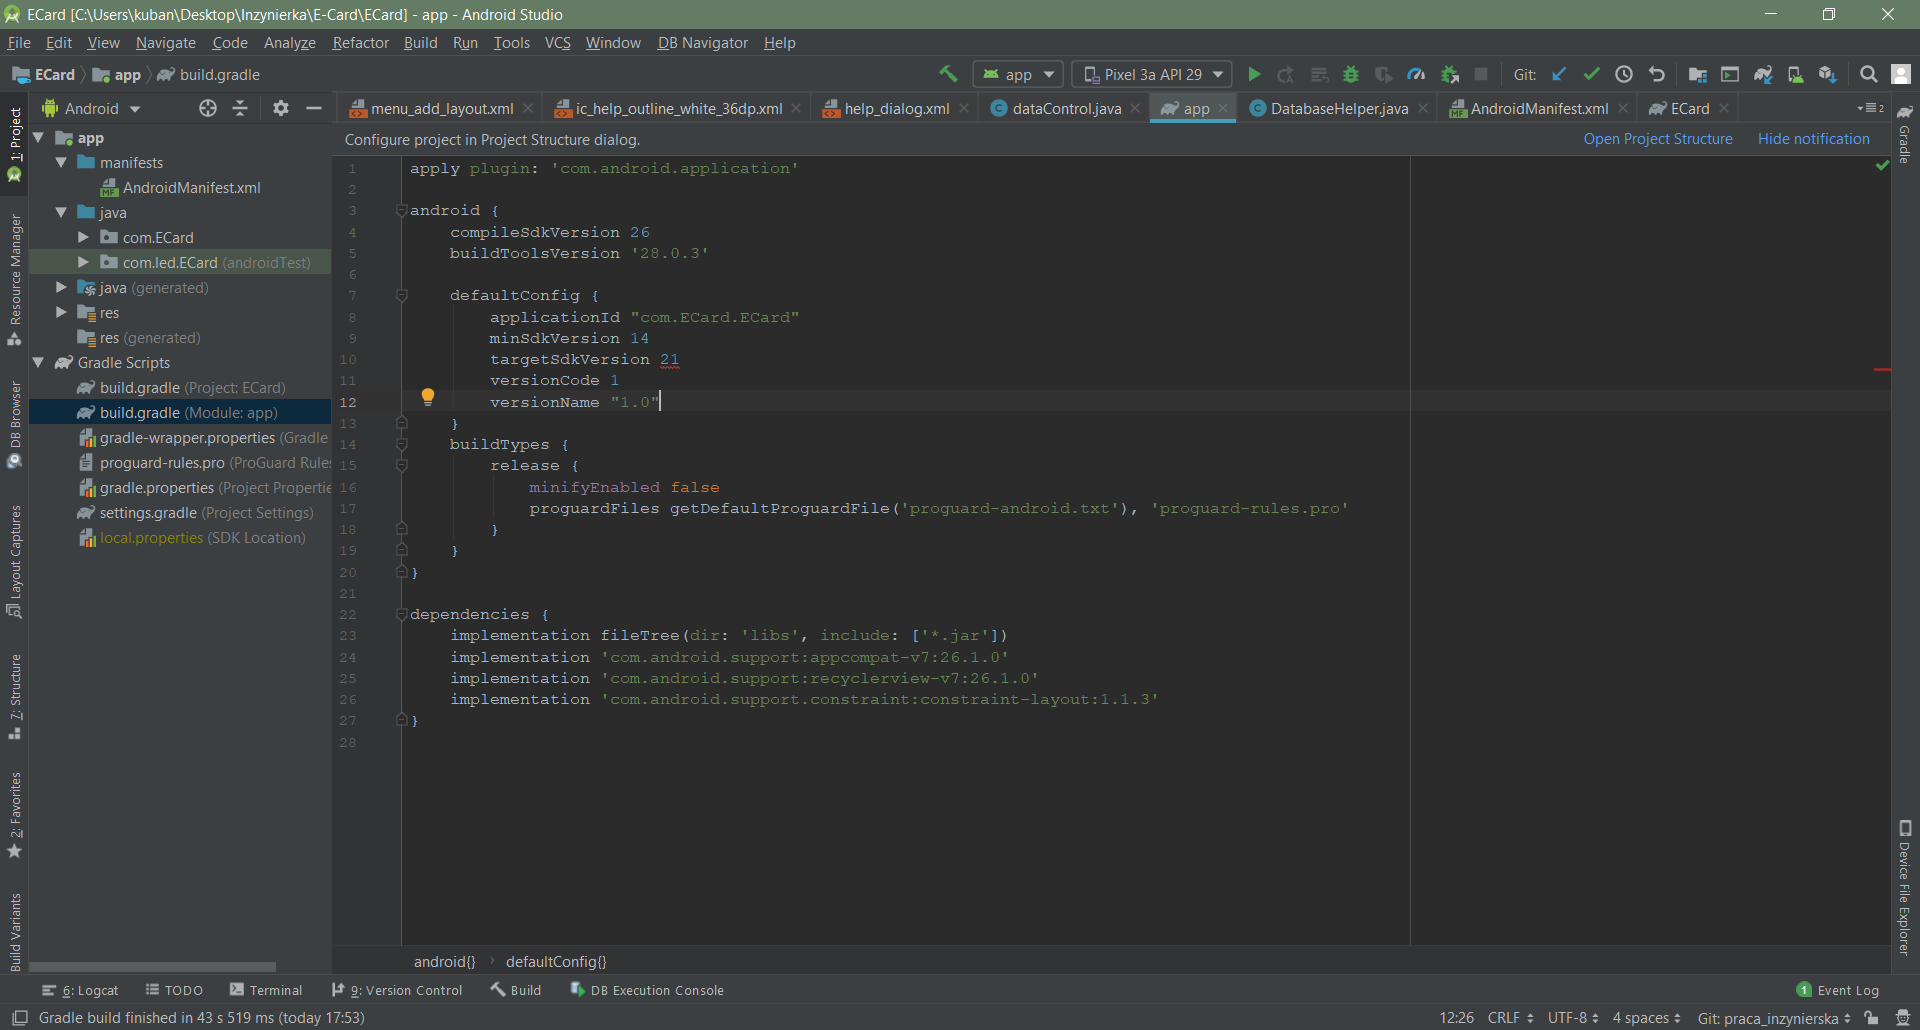
\includegraphics[width=16cm]{images/rys4_android.png}
			\vspace{.5cm}
			\caption{Widok Android Studio}
            \label{fig:androidstudio}
	\end{figure}
	
	\newpage
	\begin{flushleft}
	Oprócz posiadanie czołowych możliwości edycji kodu i wbudowanych zaawansowanych narzędzi programistycznych cechuje się również:
	\begin{itemize}
	    \item elastycznym narzędziem służącym do budowania projektów opartym na Gradle\cite{gradle}
	    \item szybkim i bogatym w funkcje emulatorem
	    \item zunifikowanym środowiskiem do produkcji aplikacji na wszystkie urządzenia z systemem android
	    \item szablonami kodu i integracją z GitHub
	    \item obszernymi narzędziami do testowania kodu i aplikacji
	    \item narzędziami do wykrywania błędów składni \textit{Lint}\cite{lint}, niezgodności wersji i innych błędów
	    \item wsparciem \textit{Native Development Kit}\cite{ndk}
	\end{itemize}
	\end{flushleft}
	\newpage
	\subsubsection{Git}
	\vspace{.5cm}
	Git jest to rozproszony system kontroli wersji stworzony przez Linusa Torvaldsa. Jest to wolne oprogramowanie opublikowane na licencji GNU GPL v2.0.
	
	Git śledzi wszelkie różnice dokonane w plikach, pozwala wrócić do dowolnej wcześniejszej wersji. Daje możliwość podglądu wszystkich zmian, które były wykonane w pliku z dokładnością to zmian w każdej linii kodu. Jest zbudowany do pracy w wiele osób, widzimy zmiany wprowadzone przez innych.
	
	Jedną z najbardziej przydatnych funkcji są gałęzie. Dzięki nim wiele osób może pracować nad różnymi funkcjonalnościami aplikacji bez przeszkadzania sobie, a następnie w prosty i szybki sposób zmiany te można dołożyć do głównej gałęzi projektu.
		\begin{figure}[H]
			\centering
			\vspace{.5cm}
			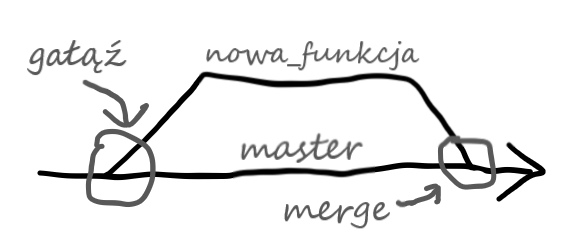
\includegraphics[width=11cm]{images/rys1_branches.png}
			\vspace{.5cm}
			\caption{Schemat wykorzystania gałęzi}
            \label{fig:branching}
		\end{figure}

	Uzyskujemy dzięki temu kontrole nad projektem, która przekłada się na mniejszą ilość błędów większą ilość czasu, którą można przeznaczyć na tworzenie nowych funkcjonalności niż na ręczne składanie kodu wielu osób.\cite{git}
	
	\newpage
	\subsubsection{GitKraken}
	\vspace{.5cm}
	GitKraken jest graficznym klientem Gita dla wielu platform zbudowanym przez AxoSoft w 2014 roku. GitKraken uproszcza skomplikowane komendy tekstowe wiersza poleceń\cite{cli} wykorzystywanego do obsługi GIT. Pozwala na korzystanie ze zdalnych repozytoriów poprzez integrację z takimi systemami jak np. GitHub, GitLab czy Bitbucket. W aplikacji wbudowane są narzędzia rozwiązywania konfliktów scalania, dostępny jest również edytor tekstowy. 
	\begin{figure}[H]
			\vspace{1cm}
			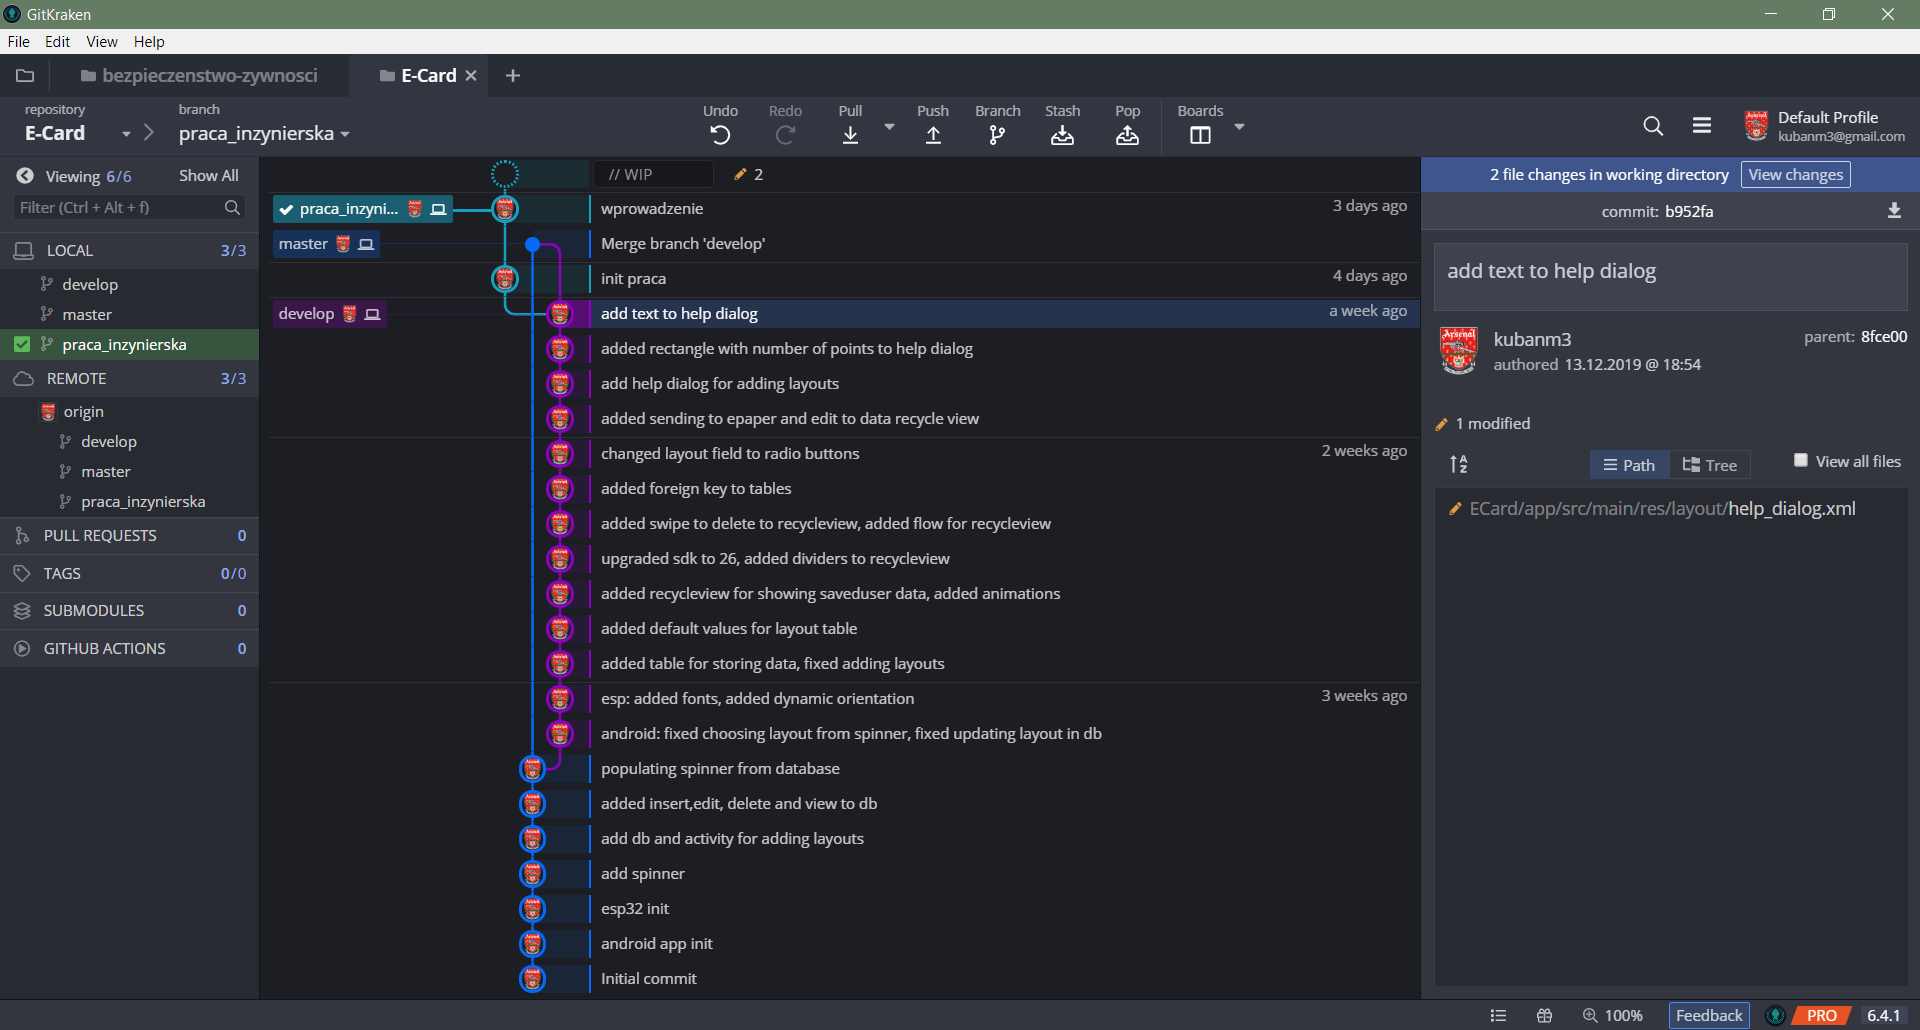
\includegraphics[width=16cm]{images/rys2_gitkraken.png}
			\vspace{.5cm}
			\caption{Repozytorium przedstawione w GitKraken}
            \label{fig:gitkraken}
	\end{figure}
		
	\vspace{.5cm}
	W projektach, gdzie pracuje jednocześnie wiele osób graficzna wizualizacja ułatwia kontrole nad wieloma gałęziami i zapanowanie nad projektem.   
	
	\newpage
	\subsubsection{Arduino IDE}
	Arduino IDE jest wieloplatformowym zintegrowanym środowiskiem deweloperskim napisanym w języku C oraz C++. Oparty jest na wolnej licencji GNU GPL v2.0. Używane jest do pisania oraz wgrywania programów do kompatybilnych płytek Arduino. Możliwe jest również wykorzystanie go do wgrywania na płytki firm trzecich za pomocą dołączonych do nich sterowników. 
	
	Programy pisane są w językach C oraz C++ używając specjalnych struktur kodowania. Udostępnionych jest na nie wiele bibliotek obsługujących szeroką gamę czujników, serw czy wyświetlaczy.
	
	\begin{figure}[H]
			\vspace{.5cm}
			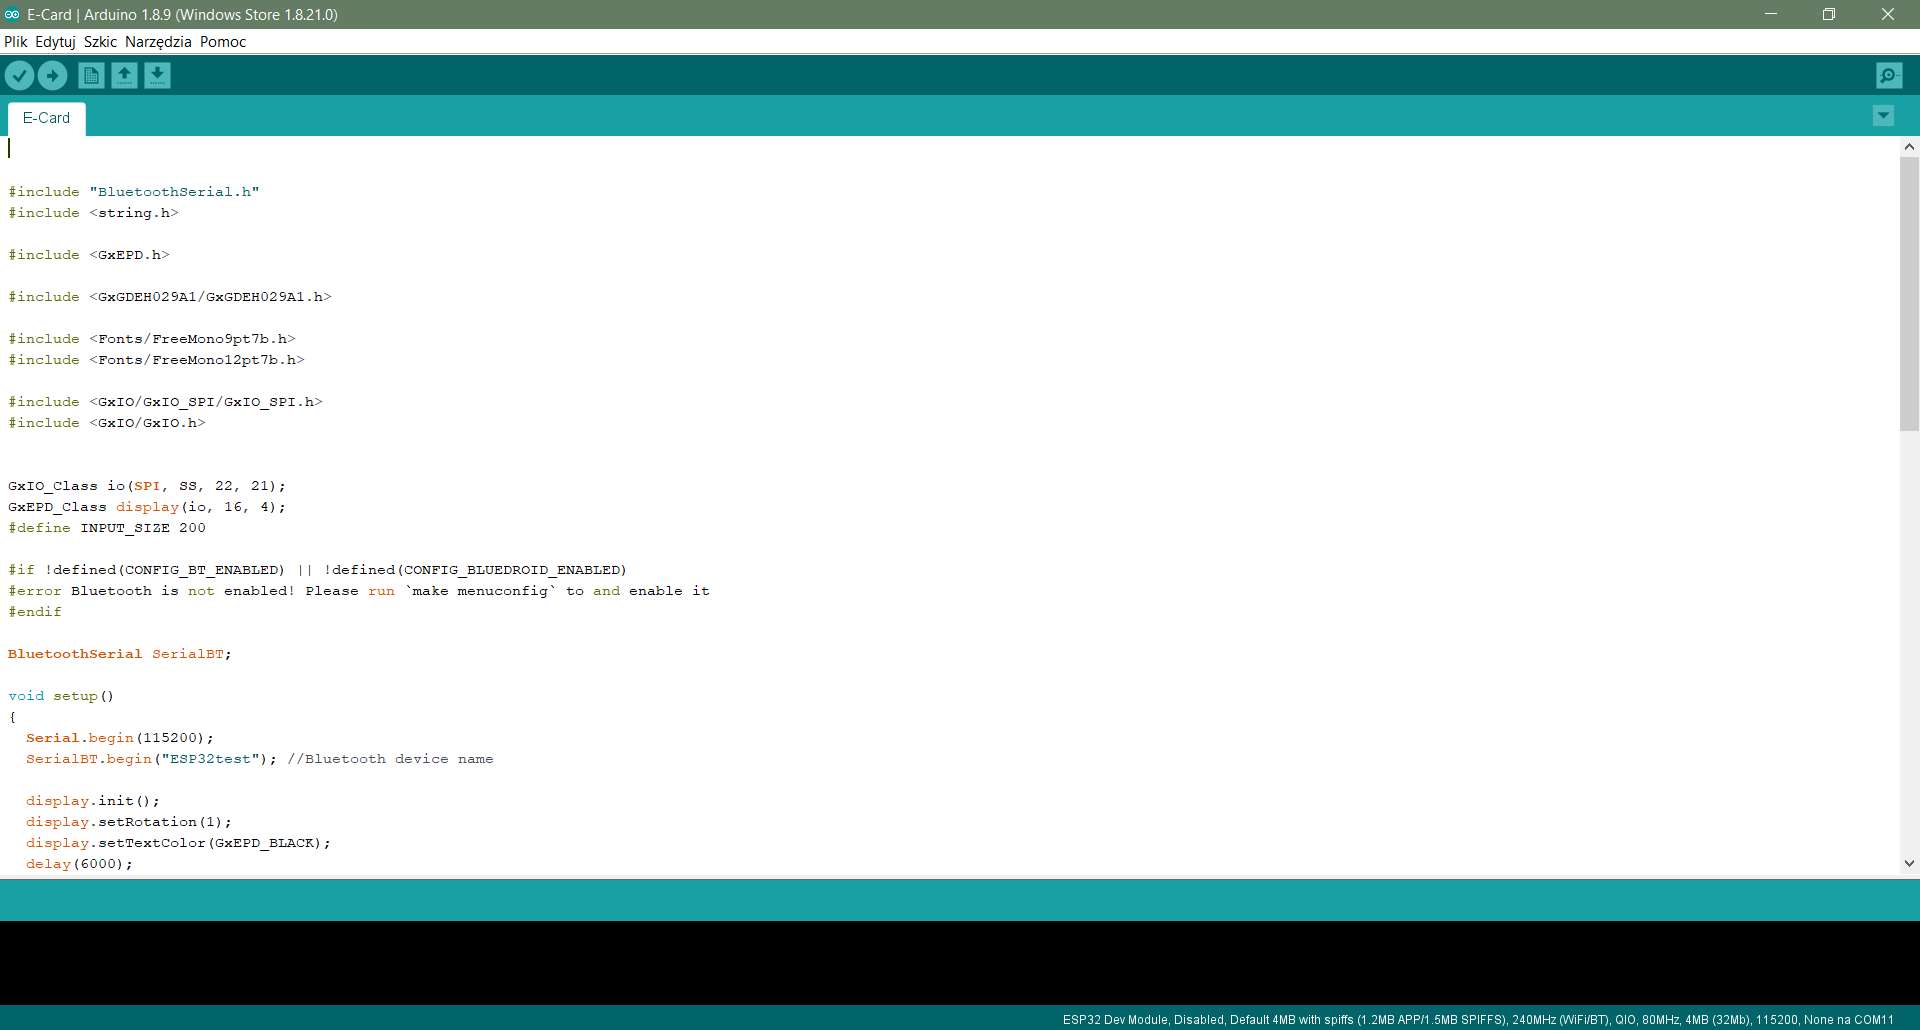
\includegraphics[width=16cm]{images/rys3_arduino.png}
			\vspace{.5cm}
			\caption{Widok Arduino IDE}
			\vspace{1cm}
            \label{fig:arduinoide}
	\end{figure}

	Napisany przez użytkownika kod do działania potrzebuje tylko dwie podstawowe funkcje. Są nimi setup() do rozpoczęcia działania i ustawienia początkowych parametrów oraz loop(), która jest pętlą główną programu.
	
	\newpage
	Środowisko zawiera trzy najważniejsze podprogramy, którymi są:
	\begin{itemize}
	\item Edytor kodu źródłowego - piszemy w nim nasz program. Zawiera takie funkcje jak sprawdzanie składni czy auto-formatowanie kodu.
	\item Kompilator - wykonuje konwersje kodu wykonywalnego w plik tekstowy z szesnastkowym kodowaniem zrozumiałym przez mikrokontroler.
	\item Loader - przesyła odpowiedni plik do Arduino.
	\end{itemize}
	
	\newpage
	\subsection{Wykorzystane technologie}
	\subsubsection{Java}
	Java jest opartym na klasach obiektowym językiem programowania. W programowaniu dla Androida wykorzystuje się przygotowane dla niego SDK\textit{ z ang. Software development kit}\cite{sdk}.
	
	W systemie Android cykl życia aplikacji wygląda inaczej niż w aplikacjach kontrolowanych przez \textit{Java Virtual Machine}\cite{jvm}. Nie występuje tutaj klasyczna metoda jaką jest \textit{public static main(String[] args) {...}} a mamy za to nowe metody w klasie aktywności jakimi są onCreate, onPause, onDestroy, onRestart i inne. Metody te wykorzystywane są w różnych momentach działania aktywności co możemy zobaczyć na rysunku \ref{fig:lifecycle}.

	
	\begin{figure}[H]
	        \centering
			\vspace{.5cm}
			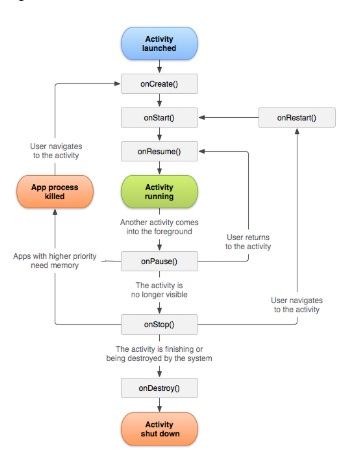
\includegraphics[width=10cm]{images/rys6_androidlifecycle.png}
			\vspace{.5cm}
			\caption{Uproszczony ilustracja cyklu życia aktywności\cite{lifecycle}}
            \label{fig:lifecycle}
	\end{figure}
	
	Metoda onCreate jest metodą uruchamianą jako pierwszą. Tutaj ustawiamy widok aktywności. W niej także przypisujemy elementy do kodu, który chcemy aby się wykonywał po interakcji z określoną kontrolką.
		
	Widoki aplikacji są budowane w wielu różnych plikach XML oraz w klasach activity, gdzie można również tworzyć elementy programowo.
	
	W przeciwieństwie do \textit{JVM} gdzie mamy pełną kontrolę nad cyklem życia procesu. W Androidzie aktywności są ciągle aktywne w tle po zamknięciu aplikacji przez użytkownika. To system steruje, kiedy aktywności zostają całkowicie wyłączone i usunięte z pamięci urządzenia. 
	
	Po zamknięciu aplikacji mogą one ciągle działać w tle jedynie zmniejszając część używanej przez siebie pamięci oraz zamknięciu niektórych z używanych procesów jak na przykład połączenie Bluetooth, GPS czy łączność z internetem. Takie rozwiązanie ma sprzyjać szybkości i zużyciu zasobów podczas ponownego uruchamiania aplikacji przez co polepszać wykorzystanie baterii\cite{batterysave}.
	
	Więcej informacji oraz większa liczba szczegółów można zaczerpnąć z książki \textit{Android Programming: The Big Nerd Ranch Guide (3rd Edition)}\cite{androidprogramming}.
	
	\vspace{1cm}
	\subsubsection{SQLite}
	SQLite jest relacyjną bazą danych dostępną na licencji \textit{public domain}\cite{publicdomain} zbudowaną w 2000 roku przez Richarda Hippa. SQLite implementuje mały rozmiarem (mniej niż 600KiB), szybki, samodzielny  silnik SQL \textit{(ang. Structured Query Language)}. Jest najczęściej używanym silnikiem baz danych na świecie. Występuje we wszystkich telefonach mobilnych oraz większości komputerów.Do działania nie potrzebuje dodatkowego procesu serwera, zapisuje i odczytuje dane bezpośrednio ze zwykłych dysków danych. Format plików jest uniwersalny, możliwe jest używanie jej i kopiowanie baz po stworzeniu pomiędzy systemami 32 lub 64 bitowymi czy wykorzystującymi architektury kolejności bajtów \textit{big-endian} lub \textit{little-endian}\cite{endian}. SQLite jest starannie testowana przed wypuszczenie każdej nowej wersji oprogramowania. Automatyczne testy osiągają 100 procent pokrycia rozgałęzień\cite{branchcoverage}. Na co dzień SQLite jest wspierany przez międzynarodowy zespół programistów pracujących nad nim w pełnym wymiarze czasu. Kod źródłowy jest otwarty i dostępny dla każdego\cite{sqlite}.
	
	Szczegółowe informacje dotyczące SQLite i jej zasad działania i użytych technologii na najniższym poziomie dostępne są w książce \textit{SQLite Forensics (2018)}\cite{sqliteforensics}. 
	
	\vspace{1cm}
	\subsubsection{Kod Arduino}
	Kod Arduino pisany jest w C++ z dołączonymi do niego specjalnymi metodami i funkcjami wykorzystywanymi i napisanymi specjalnie dla płytek Arduino i ich klonów. Ze względu na otwartą naturę projektu Arduino, biblioteki i inne zasoby posiadają obszerną liczbę pozycji. Arduino posiada wiele wbudowanych bibliotek dostarczających podstawowe funkcjonalności większości elementów, które można podłączyć do płytki. 
	
	\begin{flushleft}
	\vspace{.5cm}Programowanie programów dla Arduino jest podzielone na dwie główne części:
	\begin{enumerate}
	    \item  
	    \textbf{setup()}, ustalamy tutaj początkowy stan Arduino po uruchomieniu. Wykonywany jest tylko jeden raz.	
	    \begin{itemize}
	        \item ustalamy początkowy stan pinów
	        \item przypisujemy zmienne
	        \item tworzymy klasy
    	\end{itemize}
    	\item  
	    \textbf{loop()}, uruchamiana jest po skończeniu działania setup(). Uruchamiana jest w nieskończonej pętli. Opisana jest w niej główna logika programu.
	\end{enumerate}
	
	\flushleft\vspace{.5cm}Podstawowy zarys jak programować w Arduino można opisać w czterech krokach.\cite{stepsarduino} 
	
	
	\begin{enumerate}
	    \item \textbf{Konfiguracja} - najczęściej będzie opisana w \textit{setup()}. Wykonywana tylko raz do opisu pinów, przypisania zmiennych, kalibracji czujników.
	    \item \textbf{Dane wejściowe} - po rozpoczęciu \textit{loop()} powinniśmy przypisać przychodzące dane do zmiennych do dalszego wykorzystania lub do wywołania odpowiednich kawałków kodu zależnie od przychodzących danych, tj. jako instrukcje warunkowe.  
	    \item \textbf{Obsługa danych} - konwersja danych w łatwiejsze do obsługi przez programistę np. przypisanie danych z portu szeregowego do tablic po zastosowaniu odpowiednich kodowań. Przystosowanie danych do dalszego przesłania jeżeli wymaga tego program.
	    \item \textbf{Dane wyjściowe} - np. wysyłanie przygotowanych danych w odpowiedniej formie na port szeregowy do dalszej obróbki przez inne systemy czy przełączanie pinów na stany odpowiadające logice kodu.
	\end{enumerate}
	\end{flushleft}
	
	\vspace{1cm}
    Biblioteki wykorzystywane w programy Arduino składają się z plików źródłowych z rozszerzeniem \textit{.cpp}, oraz plików nagłówkowych \textit{.h}. Pliki nagłówkowe opisują strukturę biblioteki. Są w niej również deklarowane wszystkie zmienne i funkcje wykorzystywane przez bibliotekę. W plikach źródłowych \textit{.cpp} zawarte są implementowane kody funkcji.
    
    \vspace{1cm}
	\section{Opis i specyfikacja urządzenia}
	Elektroniczna plakietka konfigurowana z urządzenia mobilnego składa się z dwóch fizycznych części. Urządzenia mobilnego z zainstalowanym oprogramowaniem napisanym do obsługi tego projektu oraz urządzenia będącego fizyczną częścią projektu. Składającego się z mikrokontrolera oraz wyświetlacza w technologii elektronicznego papieru.

    Przedstawię w tym rozdziale ogólny schemat projektu, wybrane podzespoły do wykonania projektu, idee działania jak również algorytm, według którego działa program mikrokontrolera.
    \vspace{.5cm}
    \subsection{Opis części fizycznej projektu}
    Urządzenie wyświetlające zostało zaprojektowane do działania na mikrokontrolerze ESP32 firmy Espressif. Mikrokontroler posiada wbudowany moduł \textit{Bluetooth} BR/EDR \textit{z ang. Basic Rate/Enhanced Data Rate}\cite{edr} oraz BLE \textit{z ang. Bluetooth Low Energy}\cite{ble}, do łączenia z urządzeniem mobilnym. Do wyświetlania przesyłanych danych używany jest wyświetlacz elektronicznego papieru firmy Waveshare model WSR-09099 posiadający ekran o przekątnej 2.9 cala i rozdzielczości 296 × 128 pikseli. Możliwe jest jednak wykorzystanie dowolnego wyświetlacza 
    pracującego w szeregowym interfejsie SPI 4-line i obsługiwanego przez biblioteki \textit{GxEPD}\cite{gxepd}.
    \vspace{.5cm}
    \subsubsection{Schemat blokowy projektu}
    \begin{figure}[H]
	        \centering
			\vspace{.5cm}
			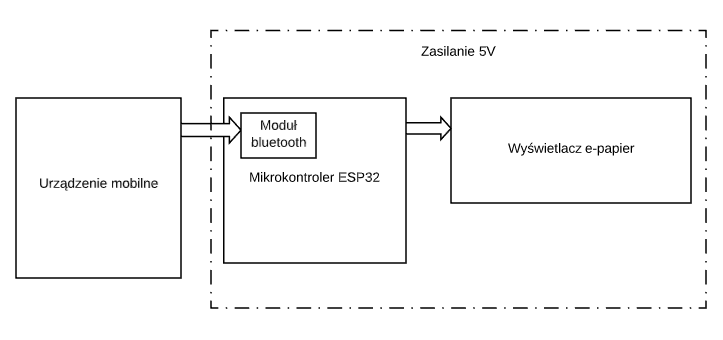
\includegraphics[width=14cm]{images/rys_7schemat_blokowy.png}
			\vspace{.5cm}
			\caption{Schemat blokowy projektu}
            \label{fig:block}
	\end{figure}
	\vspace{.5cm}
    \subsubsection{Opis poszczególnych bloków układu}
    \textbf{Urządzenie mobilne} wykorzystane do obsługi wyświetlacza papieru elektronicznego musi posiadać wersje systemu Android OS w wersji co najmniej 4.0.3 (\textit{Ice Cream Sandwich})\cite{ics}, posiadającą API w wersji 15\cite{api}. 
    
    Kolejnym wymogiem wykorzystania pełnej funkcjonalności projektu jest obecność modułu Bluetooth w urządzeniu mobilnym. Bez jego obecności nie możliwym jest przesłanie danych do mikrokontrolera a zarazem wyświetlenie ich na papierze elektronicznym.
    
    \vspace{1cm}
    
	\textbf{Mikrokontroler}, który użyto w projekcie to 32-bitowy ESP32. Pracuje on przy 3.3V napięcia roboczego. Do zbudowania prototypu posłużono się kitem developerskim ESP32-DevKitC. Posiada on wbudowany port Micro-USB do zasilania urządzenia oraz łączności ze środowiskiem programistycznym Arduino. Z tego samego portu USB zasilany jest również wyświetlacz papieru elektronicznego. Kit posiada 4MB pamięci flash\cite{flash}. Mamy do dyspozycji również trzydzieści osiem wyprowadzeń z czego dwadzieścia trzy są wyprowadzeniami GPIO\textit{z ang. general-purpose input/output}. Piny te wykorzystywane są w komunikacji pomiędzy mikroprocesorem a urządzeniami peryferyjnymi.
	\vspace{.5cm}
	\begin{figure}[H]
	        \centering
			\vspace{.5cm}
			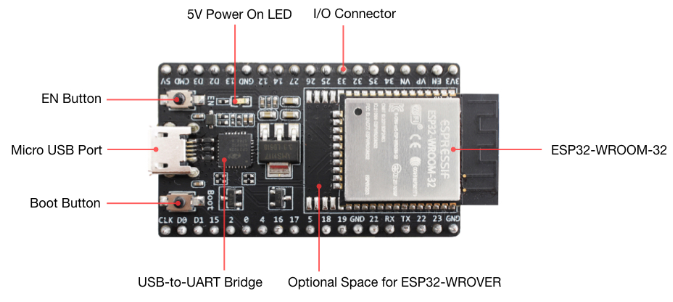
\includegraphics[width=14cm]{images/rys8_devkit.png}
			\vspace{.5cm}
			\caption{Schemat ESP32-DevKitC\cite{devkit}}
            \label{fig:devkit}
	\end{figure}
	\vspace{.5cm}
	Jego zadaniem jest odbieranie danych z połączonego urządzenia mobilnego, następnie przetworzenie ich do typu danych, z pomocą którego będzie można wysyłać je do podłączonego wyświetlacza e-papier.
	
	\vspace{1cm}

    \textbf{Wyświetlacz papieru elektronicznego} jest 2.9-cio calowym ekranem firmy Waveshare. Przystosowany jest do pracy w dwóch napięciach roboczych 3.3V oraz 5V. Zasilany jest z ESP32, który działa w 3.3V więc jest również zasilany 3.3V. Jest w stanie wyświetlać dane w dwóch kolorach (białym i czarnym) z czasem potrzebnym do odświeżenia wyświetlacza równym w przybliżeniu 0.3s\cite{waveshare}.
    
    Wykorzystane piny do połączenia wyświetlacza z mikrokontrolerem: 
    \begin{itemize}
        \item \textbf{VCC, GND} - zostały połączone z wyjściami 3.3V oraz GND mikrokontrolera. Piny te dostarczają zasilanie do wyświetlacza.
        \item \textbf{DIN, CLK, CS} - są to piny wykorzystywane przez interfejs szeregowy SPI. CLK jest linią zegara. Przez DIN dane wysyłane są z mikrokontrolera (mastera) do wyświetlacza (slave). CS używany jest do wyboru aktywnego urządzenia (stan niski), w naszym projekcie podłączone mamy tylko jedno urządzenie więc jest ono zawsze aktywne.
        \item \textbf{DC} - wybieramy czy wysyłamy dane czy komendy do wyświetlacza. Stan wysoki dla danych, stan niski dla komend
        \item \textbf{RST} - zewnętrzny reset, aktywowawny stanem niskim.
        \item \textbf{BUSY}  - linia wyjściowa wyświetlacza jest wykorzystywana do informowania mikrokontrolera o stanie zajętości wyświetlacza. Przy stanie aktywnym (aktywność przy niskim stanie) wyświetlacz nie będzie reagował na komedny przesłane przez mikrokontroler. 
    \end{itemize}
    
    \vspace{.5cm}
    \subsection{Opis części programowej mikrokontrolera}
	Program sterujący działaniem mikrokontrolera został napisany w języku C++ w zintegrowanym środowisku programistycznym Arduino IDE dostępnym za darmo na licencji GNU General Public License. Program jest kompilowany a następnie przesyłany do mikrokontrolera za pomocą wbudowanego w kit deweloperski, programatora AVRISP mk2.
	\vspace{.5cm}
	\subsubsection{Zasada działania}
	\vspace{.5cm}
    Program opiera się na dwóch częściach. Obsługa modułu Bluetooth oparta jest na kodzie napisanym przez Espressif i udostępnianym na licencji Apache License, Version 2.0. 
    
    Pierwsza część odpowiedzialna jest za upewnienie się, że moduł Bluetooth w urządzeniu sterującym działa prawidłowo.
    \vspace{1cm}
\begin{lstlisting}[language=C++, caption=Sprawdzenie poprawności działania Bluetooth]
#if !defined(CONFIG_BT_ENABLED) || !defined(CONFIG_BLUEDROID_ENABLED)
#error Bluetooth is not enabled! Please run `make menuconfig` to and enable it
#endif\end{lstlisting}
	\vspace{.5cm}
	Kolejnym korkiem jest zrobienie instancji klasy odpowiadającej za działanie modułu Bluetooth i inicjalizacja komunikacji szeregowej urządzenia sterującego z prędkością transmisji ustawioną na 115200 baudów\cite{baud}. Następnie inicjujemy szeregowe połączenie urządzenia Bluetooth i zaczynamy rozgłaszanie podanej przez nas nazwy naszego urządzenia. Po wykonaniu powyższych program przechodzi do kolejnej części.
	
	Druga część programu jest wykonywana w nieskończonej pętli. Schemat działania pętli przedstawiony jest na rysunku \ref{fig:petlamikrokontrolera}. W niej tworzymy potrzebne do działania programu zmienne i przypisujemy im startowe wartości, które później w kodzie będą modyfikowane. 
	
	Głównym zadaniem pętli jest nasłuchiwanie portu szeregowego modułu Bluetooth. Jeżeli na porcie RX modułu otrzymamy dane zapisujemy je do zmiennej. Kolejnym zadaniem wykonywanym przez nasz program jest przetworzenie otrzymanych bajtów na dane, które będzie można wysłać i wyświetlić na wyświetlaczu papieru elektronicznego. Wykorzystujemy do tego funkcję dostępną w języku C++ jaką jest \textit{strtok}\cite{strtok}. Funkcja ta rozdziela otrzymane dane z portu szeregowego Bluetooth na słowa. Ogranicznikiem, a zarazem argumentem, który musi być podany w funkcji, po którym następuje podział jest \textit{";"}. Dane wysyłane z urządzenia mobilnego są podzielone tym znakiem. 
	
	Przy pierwszym wykonaniu, funkcja oczekuje łańcucha znaków odebranego z urządzenia mobilnego jako pierwszy argument oraz znaku służącego do podziału jako drugi argument. Kolejne wywołania \textit{strtok} wykonywane są w pętli wykonującej się do otrzymania wskaźnika zerowego, który jest zwracany przez funkcję po wystąpieniu końca łańcucha znaków. Funkcja zwraca wskaźnik do następnego słowa jeżeli występowało poprzednie słowo, w wypadku gdy wystąpi koniec łańcucha znaków zwracany jest wskaźnik zerowy. W pętli kopiujemy wydzielone słowo i wpisujemy je do utworzonej wcześniej tablicy przy pomocy funkcji \textit{strcpy}\cite{strcpy}, która jest również dostępna w języku C++. Następnie wywołujemy kolejny raz \textit{strtok}, tym razem jako pierwszy argument podajemy wskaźnik zerowy. Funkcja sama ustawia się na końcu poprzedniego słowa, jako początkowe miejsce do ponownego skanowania do wykrycia znaku specjalnego. Pętla kończy się po wykryciu przez \textit{strtok} znaku \textit{null}, czyli znaku sterującego o wartości liczbowej 0, informującego o braku informacji\cite{null} i zwróceniu przez nią wskaźnika zerowego. 
	
	Pseudokod pętli pokazano w algorytmie numer \ref{lst:petlaprzepisujaca}.

\begin{lstlisting}[language=C++, label={lst:petlaprzepisujaca}, caption=Działanie pętli przepisującej otrzymane dane do tablicy]
char *ptr = strtok(input, ";");
while (ptr != NULL) {
  strcpy(ch_arr[i], ptr);
  ptr = strtok(NULL, ";");
  i++;
}\end{lstlisting}	
	\vspace{.5cm}
	Mając do dyspozycji wszystkie dane potrzebne do poprawnego wyświetlania na ekranie wyświetlacza rozpoczynamy wyświetlanie ich na ekranie. Pierwszym krokiem jest ustawienie orientacji ekranu. Następnie ustalamy wielkość czcionki oraz współrzędne pozycji startowej kursora, skąd rozpoczniemy rysowanie danych na wyświetlaczu papieru elektronicznego. Wielkość czcionki, oraz współrzędne są ustalane dla każdego tekstu wyświetlanego na ekranie papieru elektronicznego, zależnie od tego jakie informacje chcemy wyświetlić na identyfikatorze.
\vspace{1cm}
	\subsubsection{Schemat blokowy pętli programu mikrokontrolera}
	Na rysunku \ref{fig:petlamikrokontrolera} przedstawiono schemat blokowy działania głównej pętli programu mikrokontrolera ESP32. Przedstawione są tam kroki wykonywane przed wejściem do pętli oraz działanie pętli.
	
	\newpage
	\begin{figure}[H]
	        \centering
			\includegraphics[width=12cm]{images/rys10_petlamikro.png}
			\caption{Schemat blokowy pętli programu mikrokontrolera}
            \label{fig:petlamikrokontrolera}
	\end{figure}
	
	\newpage
	\section{Opis aplikacji}
	\vspace{.5cm}
	Aplikacja na urządzenie mobilne została zrobiona dla systemu mobilnego Android w środowisku Android Studio firmy Google, przystosowanej do budowy aplikacji na system Android. Aplikację napisano w języku Java. Minimalna wersja API to 15, która jest w systemie Android od wersji 4.0.3 \textit{Ice Cream Sandwich} z czerwca 2012 roku.
	
	Program został zaprojektowany zgodnie ze wzorcem programowania obiektowego\cite{oop}, w którym kod został podzielony na części, które są łatwiejsze w utrzymaniu i konserwacji. Każda część jest samodzielna w swojej funkcjonalności, zarazem możliwe jest wykorzystanie jej przez inne programy działające w aplikacji. Wszystkie części działając wspólnie tworzą całość aplikacji. Części te nazywane są obiektami. 
	
	Aplikacja posiada cztery aktywności, odpowiadające za różne funkcjonalności. Do przechowywania danych użyto relacyjnej bazy danych SQLite. W aplikacji można przechowywać zapisane dane do wyświetlenia na wyświetlaczu jak również przygotowane i zapisane układy wyświetlania.
	
	\subsection{Podział na klasy}
	Aplikacja składa się z kilku klas, są one odpowiedzialne za m.in. wyświetlanie widoku oraz obsługę jego funkcjonalności, klasa pomocnicza dla obsługi bazy danych czy klasa dla adaptera danych. Istnieje również klasa bazowa, z której dziedziczy reszty obecnych w aplikacji klas.
	
	Klasy występujące w aplikacji i ich skrócony opis:
	\begin{itemize}
	    \item \textit{DeviceList} - klasa odpowiada za sprawdzenie czy urządzenie jest wyposażone w moduł Bluetooth i czy jest on włączony. Po spełnieniu tych warunków wyświetla sparowane z urządzeniem mobilnym urządzenia Bluetooth. Po wybraniu odpowiedniego urządzenia wysyła jego adres Bluetooth \textit{z ang. Bluetooth Device Address}\cite{bdaddr} do kolejnej klasy.
	    \item \textit{DataControl} - po stworzeniu klasy następuje próba połączenia z urządzeniem, którego adres Bluetooth otrzymaliśmy, o ile urządzenie mobilne nie jest w tym samym czasie połączone. W tej samej klasie mamy pokazany widok, z którego możemy uzupełnić dane do wyświetlenia na papierze elektronicznym, po czym je bezpośrednio wysłać na urządzenie poprzez ustanowioną łączność Bluetooth lub zapisać je do bazy danych do późniejszego użycia. Została w tym miejscu również zaimplementowana funkcjonalność rozłączenia z urządzeniem Bluetooth.
	    \item \textit{DatabaseHelper} - jest to klasa pomocnicza do obsługi bazy danych SQLite. Przygotowywane i wykonywane są w niej skrypty do tworzenia tabeli dla danych oraz tabeli dla układów, która jest również uzupełniana wartościami domyślnymi. Są tutaj również napisane metody do obsługi tabel. Mamy możliwość pobrania danych rekordów z tabeli, edycji lub usunięcia ich.
	    \item \textit{DataList} - klasa, w której wyświetlane są rekordy z tabeli zawierającej zapisane dane, które można przesłać na wyświetlacz papieru elektronicznego. Po przesunięciu wybranego rekordu mamy możliwość usunięcia go lub przesłania do widoku, gdzie mamy możliwość nim sterować. Rekord można edytować lub przesłać do urządzenia, gdzie zostanie wyświetlony.
	    \item\textit{DataAdapter} - jest to klasa pomocnicza dla klasy DataList. Odpowiada ona za poprawne wyświetlanie danych pobranych z bazy danych na adapterze widoku liście.
	    \item \textit{AddLayout} - w tej klasie mamy możliwość dodawania nowych układów do wyświetlania danych na ekranie papieru elektronicznego. Klasa posiada również metody do edycji i usuwania układów danych. Jest tutaj również zaimplementowany prosty dialog pomagający w projektowaniu nowych układów, które można wyświetlać.
	    \item \textit{DynamicSquareLayout} - klasa odpowiada za obliczanie i ustawianie proporcji pomocniczego widoku wyświetlacza w dialogu pomocy zaimplementowanym w klasie \textit{AddLayout}. Proporcje te odpowiadają fizycznym rozmiarom wyświetlacza papieru elektronicznego. Wysokość i szerokość pomocniczego widoku wyświetlacza dobierane są w taki sposób, aby szerokość wyświetlacza pokazywanego w aplikacji była równa 80-ciu procentom szerokości ekranu urządzenia mobilnego.
	    \item \textit{BaseActivity} - jest klasą bazową aplikacji, z której dziedziczą inne klasy. Napisane zostały w niej metody wykorzystywane we wszystkich widokach jak również metody, które łączą kilka klas. Metodą wykorzystywaną przez wszystkie widoki a napisaną w tej klasie jest metoda odpowiedzialna za wyświetlanie wszystkich, dostępnych i zapisanych w tabeli, układów danych.
	\end{itemize}

    \subsubsection{Baza danych}
    W aplikacji istnieje możliwość przechowywania rekordów zapisanych układów oraz wpisów z danymi personalnymi do wyświetlania na identyfikatorze. Obsługa zapisanych danych wykonywana jest w relacyjnej bazie danych SQLite. Baza posiada dwie tabele połączone ze sobą kluczem obcym, na rysunku \ref{fig:database} można zobaczyć diagram związków encji bazy danych. 
    
    Kolumna id z tabeli \textit{layouts} jest kluczem głównym tej tabeli oraz jest wykorzystywana jako klucz obcy w tabeli \textit{data}. 
    
    \begin{figure}[H]
	        \centering
	        \vspace{.5cm}
			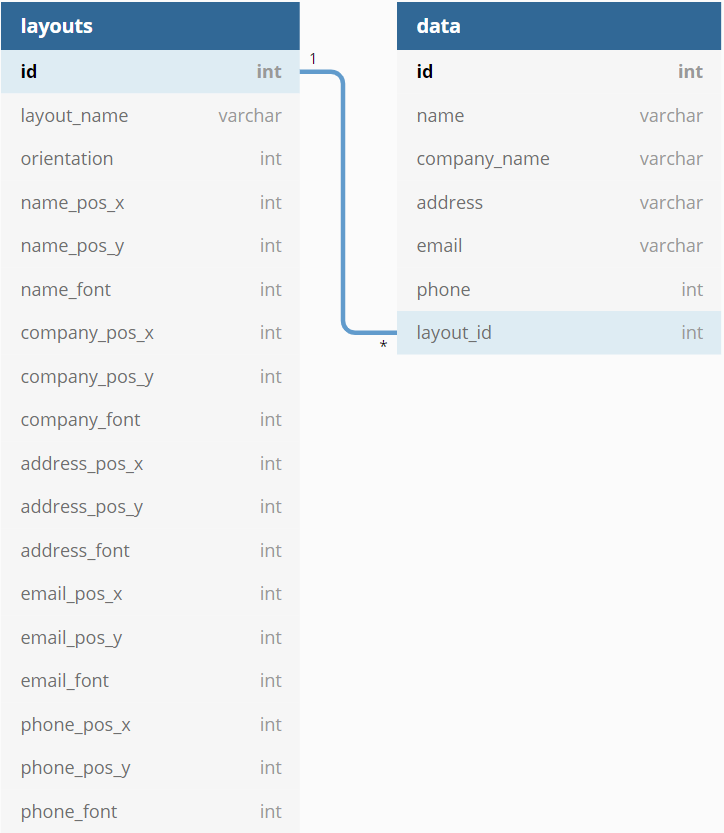
\includegraphics[width=12cm]{images/rys_11baza.png}
			\vspace{.5cm}
			\caption{Diagram związków encji bazy danych}
            \label{fig:database}
	\end{figure}
	
    Relacja pomiędzy tabelami to jeden do wielu (1:N), oznacza to, że jeden rekord tabeli \textit{layouts} może być wykorzystany przez wiele rekordów w tabeli \textit{data}. Z drugiej strony, pojedynczy wpis do tabeli \textit{data} może posiadać tylko jeden layout. Dzięki takiemu połączeniu SQLite zapewni nam poprawność działania bazy danych, uniemożliwiając usuwanie wpisów wykorzystywanych przez inne tabele. W wykorzystywanej w projekcie bazie danych, niemożliwym będzie usunięcie rekordu tabeli \textit{layouts}, gdy jego klucz główny \textit{id} jest obecny w kolumnie \textit{layout\_id} tabeli \textit{data}, który jest jednocześnie kluczem obcym tej tabeli. 
	
	\section{Instrukcja obsługi}
	\section{Podsumowanie}
	
	\newpage
	\section{Bibliografia}
	
 	\begingroup
	\renewcommand{\section}[2]{}
	\begin{thebibliography}{}
		
		\bibitem{clima_causes}
		Przyczyny zmian klimatu,
		\newline\url{https://ec.europa.eu/clima/change/causes\_pl}, 
		\newline Dostęp: 23 grudnia 2019
		
		\bibitem{cartidge_production}
		The Environmental Impact of Printer Cartridges,
		\newline\href{https://www.energycentral.com/c/ec/ink-waste-environmental-impact-printer-cartridges}
		 {\nolinkurl{https://www.energycentral.com/c/ec/}
             \\
              \nolinkurl{ink-waste-environmental-impact-printer-cartridges,}
             }
		\newline Dostęp: 24 grudnia 2019
		
		\bibitem{bluetooth}
		Bluetooth,
		\newline\url{https://pl.wikipedia.org/wiki/Bluetooth}, 
		\newline Dostęp: 27 grudnia 2019
			
		\bibitem{wifi}
		Wi-Fi,
		\newline\url{https://pl.wikipedia.org/wiki/Wi-fi}, 
		\newline Dostęp: 27 grudnia 2019
		
		\bibitem{ide}
		Zintegrowane środowisko programistyczne,
		\newline\url{https://en.wikipedia.org/wiki/Integrated_development_environment}, 
		\newline Dostęp: 28 grudnia 2019
		
		\bibitem{gradle}
		Gradle,
		\newline\url{https://docs.gradle.org/current/userguide/what_is_gradle.html}, 
		\newline Dostęp: 28 grudnia 2019
		
		\bibitem{ndk}
		Native Development Kit,
		\newline\url{https://developer.android.com/ndk}, 
		\newline Dostęp: 28 grudnia 2019
		
		\bibitem{lint}
		Lint,
		\newline\url{https://en.wikipedia.org/wiki/Lint_(software)}, 
		\newline Dostęp: 28 grudnia 2019
		
		\bibitem{git}
		Git,
		\newline\url{https://git-scm.com/book/pl/v2/Pierwsze-kroki-Wprowadzenie-do-kontroli-wersji}, 
		\newline Dostęp: 28 grudnia 2019

		\bibitem{cli}
		CLI,
		\newline\url{https://pl.wikipedia.org/wiki/CLI}, 
		\newline Dostęp: 28 grudnia 2019
		
		\bibitem{sdk}
		SDK,
		\newline\url{https://pl.wikipedia.org/wiki/Software_development_kit}, 
		\newline Dostęp: 28 grudnia 2019
		
		\bibitem{jvm}
		Wirtualna maszyna Javy,
		\newline\url{https://pl.wikipedia.org/wiki/Wirtualna_maszyna_Javy}, 
		\newline Dostęp: 28 grudnia 2019
		
		\bibitem{lifecycle}
		A simplified illustration of the activity lifecycle,
		\newline\url{https://developer.android.com/guide/components/activities/activity-lifecycle}, 
		\newline Dostęp: 28 grudnia 2019
		
	    \bibitem{batterysave}
		Wykorzystanie baterii w systemie android,
		\newline\url{https://fossbytes.com/closing-background-apps-save-battery/}, 
		\newline Dostęp: 28 grudnia 2019
		
		\bibitem{androidprogramming}
	    Bill Phillips, Chris Stewart, Kristin Marsicano, \textit{Android Programming: The Big Nerd Ranch Guide (3rd Edition)}, ISBN-13: 978-0134706054,
		\newline Data wydania: 9 luty 2017
		
	    \bibitem{publicdomain}
		Welcome to the Public Domain,
		\newline\url{https://fairuse.stanford.edu/overview/public-domain/welcome/}, 
		\newline Dostęp: 29 grudnia 2019
		
		\bibitem{endian}
		Kolejność bajtów,
		\newline\url{https://en.wikipedia.org/wiki/Endianness}, 
		\newline Dostęp: 29 grudnia 2019
		
		\bibitem{branchcoverage}
		Test Coverage,
		\newline\url{https://www.sqlite.org/testing.html#coverage}, 
		\newline Dostęp: 29 grudnia 2019
		
		\bibitem{sqlite}
		About SQLite,
		\newline\url{https://www.sqlite.org/about.html}, 
		\newline Dostęp: 29 grudnia 2019
		
		\bibitem{sqliteforensics}
	    Paul Sanderson, \textit{SQLite Forensics}, ISBN-13: 978-1980293071,
		\newline Data wydania: 12 maj 2018
		
		\bibitem{stepsarduino}
		EVERYTHING YOU NEED TO KNOW ABOUT ARDUINO CODE,
		\newline\url{https://www.circuito.io/blog/arduino-code/}, 
		\newline Dostęp: 29 grudnia 2019
		
		\bibitem{ble}
		Bluetooth Low Energy,
		\newline\url{https://web.archive.org/web/20170310111443/https://www.bluetooth.com/what-is-bluetooth-technology/how-it-works/low-energy}, 
		\newline Dostęp: 10 marca 2017
		
		\bibitem{edr}
		Bluetooth: Bluetooth BR/EDR,
		\newline\url{https://eu.industrial.panasonic.com/products/wireless-connectivity/bluetooth/bluetooth-bredr}, 
		\newline Dostęp: 3 stycznia 2020

        \bibitem{gxepd}
		GxEPD,
		\newline\url{https://github.com/ZinggJM/GxEPD}, 
		\newline Dostęp: 3 stycznia 2020
		
		\bibitem{api}
		SDK Platform release notes,
		\newline\url{https://developer.android.com/studio/releases/platforms}, 
		\newline Dostęp: 3 stycznia 2020
		
		\bibitem{ics}
		Ice Cream Sandwich,
		\newline\url{https://developer.android.com/about/versions/android-4.0-highlights}, 
		\newline Dostęp: 3 stycznia 2020
		
		\bibitem{devkit}
		ESP32-DevKitC V4 with ESP32-WROOM-32 module soldered,
		\newline\url{https://docs.espressif.com/projects/esp-idf/en/latest/hw-reference/get-started-devkitc.html}, 
		\newline Dostęp: 3 stycznia 2020
		
		\bibitem{flash}
		Zrozumieć pamięć Flash,
		\newline\url{https://mikrokontroler.pl/2018/01/26/zrozumiec-pamiec-flash/}, 
		\newline Dostęp: 3 stycznia 2020
		
		\bibitem{waveshare}
		2.9inch e-Paper Module User Manual,
		\newline\url{https://www.waveshare.com/w/upload/9/98/2.9inch-e-paper-module-user-manual-en.pdf}, 
		\newline Dostęp: 3 stycznia 2020
		
		\bibitem{baud}
		What is Baud Rate \& Why is it important?,
		\newline\url{https://www.setra.com/blog/what-is-baud-rate-and-what-cable-length-is-required-1}, 
		\newline Dostęp: 4 stycznia 2020
		
		\bibitem{strtok}
		function strtok,
		\newline\url{http://www.cplusplus.com/reference/cstring/strtok/}, 
		\newline Dostęp: 4 stycznia 2020
		
		\bibitem{strcpy}
		function strcpy,
		\newline\url{http://www.cplusplus.com/reference/cstring/strcpy/}, 
		\newline Dostęp: 4 stycznia 2020
		
		\bibitem{null}
		Null (znak),
		\newline\url{https://pl.wikipedia.org/wiki/Null_(znak)}, 
		\newline Dostęp: 4 stycznia 2020
		
		\bibitem{oop}
	    John Horton, \textit{Android Programming for Beginnersb}, Packt Publishing,
		\newline Data wydania: 31 grudnia 2015
		
		\bibitem{bdaddr}
		What is Bluetooth Address (BD\_ADDR),
		\newline\url{https://macaddresschanger.com/what-is-bluetooth-address-BD_ADDR}, 
		\newline Dostęp: 4 stycznia 2020
		
	\end{thebibliography}
	\endgroup
	
	\newpage
	\section{Spis rysunków}
	\begingroup
	\renewcommand{\section}[2]{}%
	\listoffigures
	\endgroup
	
	\newpage
	\section{Spis algorytmów}
	\begingroup
	\renewcommand{\section}[2]{}%
	\lstlistoflistings
	\renewcommand{\section}[2]{}%
	\endgroup
	
\end{document}